\documentclass{beamer}
\usetheme{Singapore}
\usecolortheme{default}

\usepackage[utf8]{inputenc}
\usepackage[T1]{fontenc}
\usepackage{verbatim}
\usepackage{graphics}
\usepackage{listings}
\usepackage{lmodern}

\title{Understanding Git with Alloy}
\subtitle{Milestone 3}
\author{Cláudio Lourenço \and Renato Neves}
\institute{University of Minho\\
Formal Methods in Software Engineering}


\logo{ 
\includegraphics[width=0.15\textwidth]{images/csail_logo.png}
       
\includegraphics[width=0.15\textwidth]{images/uminho_eng_logo.png}}

\begin{document}

\frame {
   \titlepage
}

\frame{
   \frametitle{Table of contents}
   \tableofcontents 
}

\section{Git Structure}
\begin{frame}
   \frametitle{The Git Structure}
   \begin{figure}
      \centering
      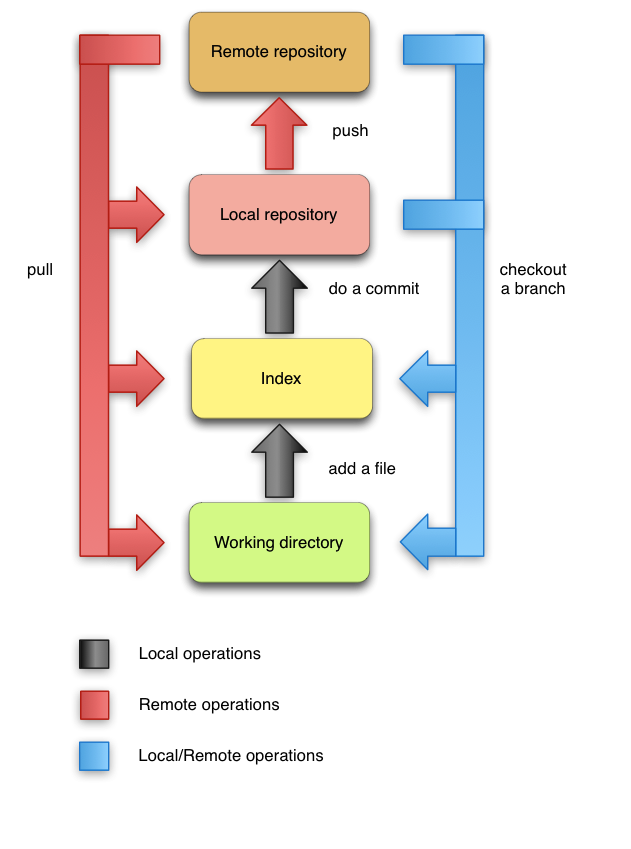
\includegraphics[width=0.5\textwidth]{images/git_workflow.png}
   \end{figure}
\end{frame}

\section{Repository}
\begin{frame}
   \frametitle{Repository}
   Esta imagem tem que ser alterada; Quadrado exterior sendo o
   repositorio, 2 quadrados internos, um para os objectos e outro para
   as referencias
   \begin{figure}
      \centering
      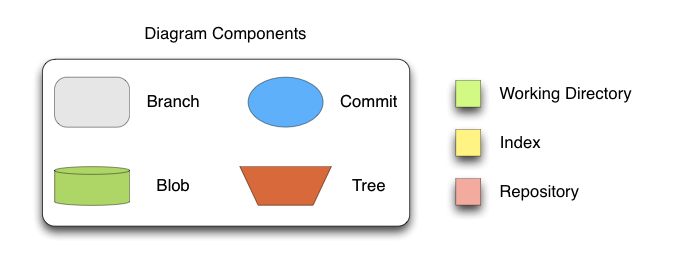
\includegraphics[width=0.8\textwidth]{images/Legenda.png}
   \end{figure}
\end{frame}

\begin{frame}[fragile]
   \frametitle{Blob and Tree}
   \begin{block}{Blob}
      \begin{itemize}
         \item Represents the content of a file;
         \item The name is calculated from its content;
      \end{itemize}
      \tiny
      \color{blue}
      \begin{lstlisting}
      sig Blob extends Object {}
      \end{lstlisting}
   \end{block}
   \begin{block}{Tree}
      \begin{itemize}
         \item Relation from names to Blobs or/and Trees;
         \item Used to represent the file system structure;
      \end{itemize}
      \tiny
      \color{blue}
      \begin{lstlisting}
      sig Tree extends Object {
         
         contains: Name -> lone(Tree+Blob)
      
      }
      \end{lstlisting}
   \end{block}
\end{frame}


\begin{frame}[fragile]
   \frametitle{Commit}
   \begin{itemize}
      \item It is like a snapshot of the project on a certain moment
      in time;
      \item Author, Committer, Comment - Not important for us;
      \item Parent - The Commit which originated the current;
      \item Tree - Pointer to a Tree Object;
   \end{itemize}
   \tiny
   \color{blue}
   \begin{lstlisting}
                        sig Commit extends Object {
                           points : Tree,
                           parent : set Commit,
                           abs: Path -> Object,
                           merge : set State
                        }
                           
                        sig RootCommit extends Commit {}
\end{lstlisting}
\end{frame}

\begin{frame}[fragile]
\frametitle{Branch and HEAD}
   \begin{block}{Branch}
      \begin{itemize}
         \item It is just a pointer to a commit;
      \end{itemize}
   \end{block}
   \begin{block}{HEAD}
      \begin{itemize} 
         \item Special reference that identifies the current Branch;
      \end{itemize}
   \end{block}
   \tiny
   \color{blue}
   \begin{lstlisting}
                        sig Branch{
                           marks: Commit lone -> State,
                           branches: set State,
                           head: set State
                        }

                        lone sig Master extends Branch{}
   \end{lstlisting}
\end{frame}


\section{Working Directory}
\begin{frame}
   \frametitle{Working Directory}
\end{frame}

\section{Index}
\begin{frame}
   \frametitle{Index}
\end{frame}

\section{Operations}
\begin{frame}
   \frametitle{Operations}
\end{frame}

\end{document}
